\documentclass{hrumc}

\usepackage{lipsum}
\begin{document}
\newgeometry{left=1.25in,right=1.25in,bottom=1in,top=1in}
\onecolumn

% ----------------------------
% front cover
\vspace*{2ex plus 1fil}
\fronttitle{XXIII}
\vspace*{5ex plus 1fil}
\begin{frontgraphic}
  \put(0,-.25){\makebox[0em]{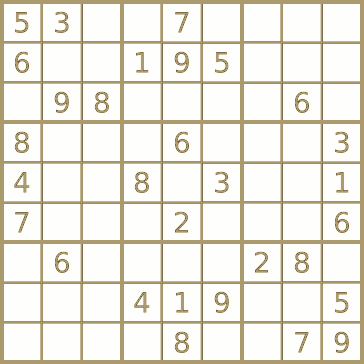
\includegraphics[scale=0.6]{sodoku.png}}}
  \put(0,-0.11){\makebox[0em]{
\includegraphics[scale=0.54]{pnp.png}}} % http://news.mit.edu/2009/explainer-pnp
\end{frontgraphic}
\vspace*{5ex}
\frontfoot
\vspace*{2ex plus 1fil}
\clearpage



% ----------------------------
% inside cover
\begin{scheduleoverview}
  8:30  &9:50am  &Registration             &Dion Center              \\
  10:00 &10:55am &Parallel Sessions One     &St~Edmunds and Jeanmarie Halls \\
  11:05 &12:15pm &Welcome, Invited Address  &McCarthy Arts Center     \\
  12:25 &1:30pm  &Lunch                     &Dion Center              \\
  1:40  &2:55pm  &Parallel Sessions Two     &St~Edmunds and Jeanmarie Halls \\
  3:00  &3:25pm  &Coffee and refereshments  &Dion Center  \\
  3:30  &4:25pm  &Parallel Sessions Three   &St~Edmunds and Jeanmarie Halls
\end{scheduleoverview}
\vspace{2ex plus 1 fill}
\wifi{guest}{guest}
\fullprogram{http://joshua.smcvt.edu/hrumc/full.pdf}
\vspace*{4ex}
\begin{help}
      \item[Medical, fire, or police]
       In an emergency call 911. 
       For non-emergency security or safety issues, call campus 
       security at 802-654-2911, or simply dial 2911 from any campus phone. 
       There is a campus phone in each classroom.

    \item[Classroom equipment]
      There will be student assistants, wearing special tee-shirts, 
      in or near each classroom to help with  
      computers or other equipment.

    \item[Rest rooms]
      There are rest rooms on each floor of the academic building.
      There is a unisex rest room on the second floor of Jeanmarie,
      next to room 277.
\end{help}
\clearpage


% ----------------------------
% welcome page
{\setlength{\parskip}{1.5ex}
\setlength{\parindent}{0ex}
\welcome{twenty third}{Westfield State College}

\vspace{2ex plus 1fil}
\support{This conference would not be possible without the generous 
financial 
support provided by the Office of the Vice President for Academic Affairs 
at Saint Michael's College, and by the Departments of Mathematics and
Computer Science.
Support also comes from the NASA-VT Space Grant Consortium,
and from the Pi Mu Epsilon national Mathematics honor society.}

\vspace{2ex plus 1fil}
\begin{minipage}{\textwidth}
  \begin{hrumcsteering}
  Lauren Childs, Williams College        \\
  Paul Friedman, Union College           \\
  Mohammad Javaheri, Siena College       \\
  Emelie Kenney, Siena College           \\
  Joe Kirtland, Marist College           \\
  Allison Pacelli, Williams College      \\
  Alejandro Sarria, Williams College     \\
  David Vella, Skidmore College          \\
  William Zwicker, Union College
  \end{hrumcsteering}
  \hspace{5em plus 1fill}
  \begin{localsteering}
  Jim Hef{}feron \\
  Lloyd Simons  
  \end{localsteering}
\end{minipage}
}
\clearpage


% ----------------------------
% plenary address page
\plenaryhead{Dr.~Karen Talentino, VPAA, Saint Michael's College}{Jane Doe, SMC '17}
\vspace*{5ex}
\begin{plenary}{The $\mathbf{P}$ vs.\ $\mathbf{NP}$ Problem}{Scott Aaronson}{MIT, University of Texas at Austin}{Scott Aaronson 
holds a PhD in Computer Science from University of California, Berkeley.
He is currently Associate Professor of Electrical Engineering and 
Computer Science
at the Massachussets Institute of Technology. 
Starting in July he will be the 
David J.~Bruton Jr.\ Centennial Professor of Computer Science at the 
University of Texas at Austin. 
He has an international reputation as an expert in the Theory of Computation 
and Complexity Theory.

Scott studies the fundamental limits on what can be efficiently computed in the physical world. This entails studying quantum computing, the most powerful model of computation that we have. His work has included limitations of quantum algorithms in the black-box model; the learnability of quantum states; quantum proofs and advice; the power of postselected quantum computing and quantum computing with closed timelike curves; and linear-optical quantum computing.}

I'll discuss the status of the famous $\mathbf{P}\mathbin{\hbox{?=}}\mathbf{NP}$ 
problem in 2016, offering
a personal perspective on what it's about, why it's important, why
many experts conjecture that $\mathbf{P}\mathbin{\hbox{!=}}\mathbf{NP}$ is both true and provable, why
proving $\mathbf{P}\mathbin{\hbox{!=}}\mathbf{NP}$ is so hard, the landscape of related problems, and
crucially, what progress has been made in the last half-century.  I'll
say something about diagonalization and circuit lower bounds; the
relativization, algebrization, and natural proofs barriers; and the
recent works of Ryan Williams and Ketan Mulmuley, which (in different
ways) hint at a duality between impossibility proofs and algorithms.
\end{plenary}
\vspace*{1ex plus 1fill}


\restoregeometry




% ===== BEGIN PARALLEL SESSIONS (leave this string; it is used by hrumc.py)


\sessionhead{One}
\session{Algebra III}{STE 106}{Fred McGuilicuddy1}
\at{\Ia}{input/afinogenov}
\at{\Ib}{input/barrett}
\at{\Ic}{input/bassette}

\session{Algebra III}{STE 106}{Fred McGuilicuddy}
\at{\Ia}{input/bennett}
\at{\Ib}{input/blue}
\at{\Ic}{input/buck}

\session{Algebra III}{STE 106}{Fred McGuilicuddy}
\at{\Ia}{jones1}
\at{\Ib}{jones1}
\at{\Ic}{jones1}

\session{Algebra III}{STE 106}{Fred McGuilicuddy}
\at{\Ia}{jones1}
\at{\Ib}{jones1}
\at{\Ic}{jones1}

\session{Algebra III}{STE 106}{Fred McGuilicuddy}
\at{\Ia}{jones1}
\at{\Ib}{jones1}
\at{\Ic}{jones1}

\session{Algebra III}{STE 106}{Fred McGuilicuddy}
\at{\Ia}{jones1}
\at{\Ib}{jones1}
\at{\Ic}{jones1}

\session{Algebra III}{STE 106}{Fred McGuilicuddy}
\at{\Ia}{jones1}
\at{\Ib}{jones1}
\at{\Ic}{jones1}

\session{Algebra III}{STE 106}{Fred McGuilicuddy}
\at{\Ia}{jones1}
\at{\Ib}{jones1}
\at{\Ic}{jones1}

\session{Algebra III}{STE 106}{Fred McGuilicuddy}
\at{\Ia}{jones1}
\at{\Ib}{jones1}
\at{\Ic}{jones1}

\session{Algebra III}{STE 106}{Fred McGuilicuddy}
\at{\Ia}{jones1}
\at{\Ib}{jones1}
\at{\Ic}{jones1}






\sessionhead{Two}
\session{Algebra III}{STE 106}{Fred McGuilicuddy}
\at{\IIa}{jones1}
\at{\IIb}{jones1}
\at{\IIc}{jones1}

\session{Algebra III}{STE 106}{Fred McGuilicuddy}
\at{\IIa}{jones1}
\at{\IIb}{jones1}
\at{\IIc}{jones1}

\session{Algebra III}{STE 106}{Fred McGuilicuddy}
\at{\IIa}{jones1}
\at{\IIb}{jones1}
\at{\IIc}{jones1}

\session{Algebra III}{STE 106}{Fred McGuilicuddy}
\at{\IIa}{jones1}
\at{\IIb}{jones1}
\at{\IIc}{jones1}

\session{Algebra III}{STE 106}{Fred McGuilicuddy}
\at{\IIa}{jones1}
\at{\IIb}{jones1}
\at{\IIc}{jones1}

\session{Algebra III}{STE 106}{Fred McGuilicuddy}
\at{\IIa}{jones1}
\at{\IIb}{jones1}
\at{\IIc}{jones1}

\session{Algebra III}{STE 106}{Fred McGuilicuddy}
\at{\IIa}{jones1}
\at{\IIb}{jones1}
\at{\IIc}{jones1}

\session{Algebra III}{STE 106}{Fred McGuilicuddy}
\at{\IIa}{jones1}
\at{\IIb}{jones1}
\at{\IIc}{jones1}

\session{Algebra III}{STE 106}{Fred McGuilicuddy}
\at{\IIa}{jones1}
\at{\IIb}{jones1}
\at{\IIc}{jones1}

\session{Algebra III}{STE 106}{Fred McGuilicuddy}
\at{\IIa}{jones1}
\at{\IIb}{jones1}
\at{\IIc}{jones1}





\sessionhead{Three}
\session{Algebra III}{STE 106}{Fred McGuilicuddy}
\at{\IIIa}{jones1}
\at{\IIIb}{jones1}
\at{\IIIc}{jones1}

\session{Algebra III}{STE 106}{Fred McGuilicuddy}
\at{\IIIa}{jones1}
\at{\IIIb}{jones1}
\at{\IIIc}{jones1}

\session{Algebra III}{STE 106}{Fred McGuilicuddy}
\at{\IIIa}{jones1}
\at{\IIIb}{jones1}
\at{\IIIc}{jones1}

\session{Algebra III}{STE 106}{Fred McGuilicuddy}
\at{\IIIa}{jones1}
\at{\IIIb}{jones1}
\at{\IIIc}{jones1}

\session{Algebra III}{STE 106}{Fred McGuilicuddy}
\at{\IIIa}{jones1}
\at{\IIIb}{jones1}
\at{\IIIc}{jones1}

\session{Algebra III}{STE 106}{Fred McGuilicuddy}
\at{\IIIa}{jones1}
\at{\IIIb}{jones1}
\at{\IIIc}{jones1}

\session{Algebra III}{STE 106}{Fred McGuilicuddy}
\at{\IIIa}{jones1}
\at{\IIIb}{jones1}
\at{\IIIc}{jones1}

\session{Algebra III}{STE 106}{Fred McGuilicuddy}
\at{\IIIa}{jones1}
\at{\IIIb}{jones1}
\at{\IIIc}{jones1}

\session{Algebra III}{STE 106}{Fred McGuilicuddy}
\at{\IIIa}{jones1}
\at{\IIIb}{jones1}
\at{\IIIc}{jones1}

\session{Algebra III}{STE 106}{Fred McGuilicuddy}
\at{\IIIa}{jones1}
\at{\IIIb}{jones1}
\at{\IIIc}{jones1}

% ===== END PARALLEL SESSIONS (leave this string; it is used by hrumc.py)

% Back page is a campus map
\clearpage
\vspace*{0ex plus 1 fill}
\begin{map}[map.png]\large
    \begin{picture}(7.681,8.194)  % map is 7.681 by 8.194 inches
      \put(0,0){\usebox{\mapbox}}
      \put(-.2,1.4){\mapkey{1}{I-89 Exit 15 is a quarter mile this way}}
      \put(-.2,1.05){\mapkey{2}{Enter here, park on your left}}
      \put(-.2,.7){\mapkey{3}{McCarthy Arts building; invited address}}
      \put(-.2,.35){\mapkey{4}{Saint Edmunds Hall (STE); parallel sessions}}
      \put(-.2,.0){\mapkey{5}{Jeanmarie Hall (JEM); parallel sessions}}
      \put(-.2,-0.35){\mapkey{6}{Dion Center; register, lunch, and break}}
      \put(1,8){\circled{1}}
      \put(1.6,5.3){\circled{2}}
      \put(2.6,4.8){\circled{3}}
      \put(2.55,3.7){\circled{4}}
      \put(1.56,3.7){\circled{5}}
      \put(4,3.5){\circled{6}}
    \end{picture}   
\end{map}
\vspace*{0ex plus 1fill}

\end{document}
